\documentclass[conference]{IEEEtran}

\usepackage{cite}
\usepackage{amsmath,amssymb,amsfonts}
\usepackage{graphicx}
\usepackage{textcomp}
\usepackage{xcolor}
\usepackage{hyperref}
\usepackage{listings}
\usepackage{booktabs}
\usepackage{tikz}
\usetikzlibrary{shapes.geometric,shadows,decorations.pathmorphing}

\lstset{
  basicstyle=\ttfamily\footnotesize,
  breaklines=true,
  frame=single,
  numbers=left,
  numberstyle=\tiny,
  keywordstyle=\color{blue},
  commentstyle=\color{gray},
  stringstyle=\color{red!70!black},
}

\begin{document}

\title{A Composable Four-Gate DevSecOps Pipeline for Python:\\
Integrating SAST, Secret Detection, AST Analysis, and Dependency Auditing}

\author{
  \IEEEauthorblockN{Ali Murtaza Bhutto}
  \IEEEauthorblockA{
    \textit{Independent Security Researcher}\\
    ORCID: 0009-0007-2787-943X\\
    \href{mailto:alibhutto101112@gmail.com}{alibhutto101112@gmail.com}
  }
}

\maketitle

\begin{abstract}
Modern Python applications face a diverse threat landscape encompassing
injection vulnerabilities, inadvertently committed secrets, weak cryptographic
primitives, and transitively vulnerable dependencies. Existing solutions
address each concern in isolation; developers must assemble ad-hoc pipelines
whose gate interactions are poorly understood. We present \emph{secure-python-pipeline},
a composable, open-source DevSecOps template that chains four automated
security gates---Semgrep (SAST), Trufflehog v3 (secret detection), Bandit
(Python AST analysis), and pip-audit (dependency CVE auditing)---into a
reproducible GitHub Actions workflow. We evaluate the pipeline against five
widely-adopted OSS Python projects (httpie, rich, FastAPI, black, ruff)
totalling over 230\,000 GitHub stars, running every gate live against pinned
release tags. The dependency-CVE and secret-leak gates pass cleanly on every
project; the SAST gate surfaces between 1 and 12 findings per project, every
one of which we manually classify as a true positive, intentional design
choice, or test-fixture false-positive. The template ships with eight
CWE-mapped custom Semgrep rules, a self-test corpus that proves every rule
fires, a reference FastAPI application demonstrating correct mitigations
(parameterised SQL, bcrypt password hashing, HMAC-signed bearer tokens,
TOCTOU-safe user creation), and a local-execution script that mirrors the
CI environment.
\end{abstract}

\begin{IEEEkeywords}
DevSecOps, SAST, Python security, Semgrep, Bandit, secrets detection,
dependency auditing, CI/CD, OWASP Top 10, CWE
\end{IEEEkeywords}

%% ─────────────────────────────────────────────────────────────────────────────
\section{Introduction}

Software supply-chain attacks increased 742\% between 2019 and 2022~\cite{sonatype2022}.
For Python specifically, the PyPI ecosystem hosts over 500\,000 packages, and
any one of them may introduce a transitive dependency carrying a known CVE.
Simultaneously, OWASP's 2021 Top Ten~\cite{owasp2021} continues to list
injection (A03) and identification failures (A07) among the most prevalent
web-application risks---vulnerabilities that are, in principle, detectable
through static analysis before deployment.

Despite the availability of individual tools such as Bandit~\cite{bandit},
Semgrep~\cite{semgrep}, Trufflehog~\cite{trufflehog}, and pip-audit~\cite{pipaudit},
no reference architecture exists that: (a)~chains all four into a single
actionable workflow with documented gate-interaction semantics; (b)~ships
with a correctly-secured reference application that passes every gate;
(c)~includes a self-test corpus that proves the custom rules fire; and
(d)~empirically evaluates the pipeline against real-world OSS Python code.

This paper makes the following contributions:

\begin{enumerate}
  \item A four-gate pipeline architecture with documented gate ordering,
        failure semantics, and a fast PR-feedback workflow (\S\ref{sec:design}).
  \item Eight CWE-mapped Semgrep rules covering Python-specific OWASP Top 10
        patterns (\S\ref{sec:rules}), each verified by an automated self-test.
  \item A reference FastAPI application implementing parameterised SQL,
        bcrypt password hashing, HMAC-signed bearer-token authorisation, and
        TOCTOU-safe user creation, with 25 passing unit tests (\S\ref{sec:example}).
  \item An empirical evaluation against five high-profile OSS projects with
        complete reproducibility (\S\ref{sec:eval}).
\end{enumerate}

%% ─────────────────────────────────────────────────────────────────────────────
\section{Background and Related Work}
\label{sec:background}

\subsection{Static Application Security Testing}

SAST tools analyse source code without executing it. Semgrep~\cite{semgrep}
expresses rules as structural patterns over an AST, achieving near-zero
false-negative rates on syntactically exact matches. Bandit~\cite{bandit}
applies Python-specific heuristics (e.g., subprocess with \texttt{shell=True},
use of \texttt{pickle}) via an AST visitor, reporting severity and confidence
independently.

\subsection{Secret Detection}

Trufflehog v3~\cite{trufflehog} scans git history using entropy heuristics and
over 800 regex-based detectors, then attempts live validation to confirm that
a candidate secret is currently active. Only \emph{verified} secrets fail the
pipeline by default, dramatically reducing false-positive noise. The trade-off
is that revoked-but-leaked secrets are not flagged; teams should periodically
audit history without \texttt{--only-verified}.

\subsection{Software Composition Analysis}

pip-audit~\cite{pipaudit} queries the Python Packaging Advisory Database
(PyPA) and the OSV database for CVEs affecting pinned dependencies. Unlike
\texttt{safety}, it accepts a \texttt{requirements.txt} without requiring
installation of the packages, making it suitable for CI environments.

\subsection{Prior Work}

Pashchenko et al.~\cite{pashchenko2018} study vulnerable OSS dependencies in
npm; Decan et al.~\cite{decan2018} extend this to PyPI, finding that 11\% of
packages transitively depend on a known-vulnerable release. Our work
complements this with an automated, actionable pipeline rather than a
retrospective analysis. Zahan et al.~\cite{zahan2022} propose a threat
model for supply-chain attacks; our pipeline operationalises their
recommended controls at the CI layer. Morrison et al.~\cite{morrison2018}
examine the operational challenges of vulnerability prediction in industry,
which motivates the graduated-enforcement design of \S\ref{sec:design}.

%% ─────────────────────────────────────────────────────────────────────────────
\section{Threat Model}
\label{sec:threat}

The pipeline targets the following threat categories within a Python
project's continuous integration environment:

\textbf{T1 -- Source-level injection.} An attacker (or negligent developer)
introduces code that constructs SQL queries, shell commands, or HTTP
requests from unvalidated input. Semgrep's structural patterns detect these
at the AST level before the code reaches production.

\textbf{T2 -- Credential leakage.} A secret (API key, private key, database
password) is committed to version control, either in the current working
tree or in a past commit. Trufflehog scans the entire git history with
\texttt{fetch-depth: 0}; the \texttt{--only-verified} flag suppresses
unconfirmed candidates by attempting live validation against the issuing
service. Revoked-yet-leaked credentials are not flagged by this default
configuration; we recommend a quarterly audit without
\texttt{--only-verified} to cover that residual risk.

\textbf{T3 -- Insecure cryptographic primitives.} Passwords hashed with MD5
or SHA-1 can be inverted at sub-cent cost on modern GPU clusters. Bandit
and the project-local Semgrep rule \texttt{ali-weak-password-hash} flag
these at ERROR severity.

\textbf{T4 -- Vulnerable transitive dependencies.} A dependency introduced
for unrelated functionality may carry a CVE that is exploitable in the
project's deployment context. pip-audit resolves the full dependency graph
from \texttt{requirements*.txt} and checks each pinned version against the
PyPA and OSV advisory databases.

\textbf{Out of scope.} Runtime exploitation (memory corruption, race
conditions in C extensions), social-engineering attacks on the developer,
and adversarial model inputs in ML pipelines are explicitly excluded. The
pipeline operates purely on static artefacts.

%% ─────────────────────────────────────────────────────────────────────────────
\section{Pipeline Design}
\label{sec:design}

\subsection{Gate Ordering and Parallelism}

The four gates run in parallel as separate GitHub Actions jobs, then
converge on a summary job. This minimises wall-clock time and isolates
gate failures: an outage of the Trufflehog action does not block the
Bandit gate from completing.

\begin{enumerate}
  \item \textbf{Gate 1 -- Semgrep (SAST).} Structural AST matching catches
        injection sinks, insecure deserialisation, and debug flags. Runs
        in a pinned container (\texttt{returntocorp/semgrep:1.96.0}) for
        reproducibility, with the public \texttt{p/owasp-top-ten} and
        \texttt{p/python} rule packs plus the eight project-local rules.
  \item \textbf{Gate 2 -- Trufflehog v3 (secrets).} Scans the full git
        history (\texttt{fetch-depth: 0}). Path exclusions for test
        fixtures are configured via \texttt{.trufflehog/exclude-paths.txt}.
  \item \textbf{Gate 3 -- Bandit (Python AST).} Complements Semgrep with
        Python-semantic checks that require type information (e.g., SSL
        context verification disabled, weak hash algorithm selection).
        The gate fails only on MEDIUM- or HIGH-severity findings.
  \item \textbf{Gate 4 -- pip-audit (dependencies).} Audits every
        \texttt{requirements*.txt} file. The \texttt{--strict} flag is
        \emph{not} used: it would fail the gate on any advisory without a
        fixed version, making the badge permanently red over time when an
        unfixable CVE is disclosed in a transitive dependency.
\end{enumerate}

\subsection{Failure Semantics}

All ERROR-severity findings fail the pipeline immediately. WARNING-severity
Semgrep findings (e.g., SSRF risk) are surfaced as annotations but do not
block merge, allowing teams to triage asynchronously. This two-tier approach
follows the principle of \emph{graduated enforcement}~\cite{morrison2018}:
forcing every WARNING to block merge causes developers to globally suppress
the rule, which is worse than not having the rule at all.

\subsection{Configuration and Reproducibility}

Each gate is pinned to an exact tool version
(\texttt{bandit==1.8.6}, \texttt{pip-audit==2.10.0},
\texttt{returntocorp/semgrep:1.96.0}) so that CI results are reproducible
across machines and over time. The \texttt{bandit.yml} configuration excludes
\texttt{eval/cloned\_repos/} (vendored OSS code) and \texttt{.venv/} to avoid
noise from third-party artefacts. Trufflehog's exclude-paths file lists
\texttt{example-project/tests/fixtures/}, which contains intentionally fake
secrets used by tests, plus the \texttt{eval/semgrep\_corpus.py} self-test
corpus.

\subsection{Local Execution}

The \texttt{scripts/local\_scan.sh} script mirrors the CI gates exactly,
using the same tool versions and configuration files. Developers can run the
full pipeline locally in under two minutes on a typical codebase.

\begin{figure}[h]
  \centering
  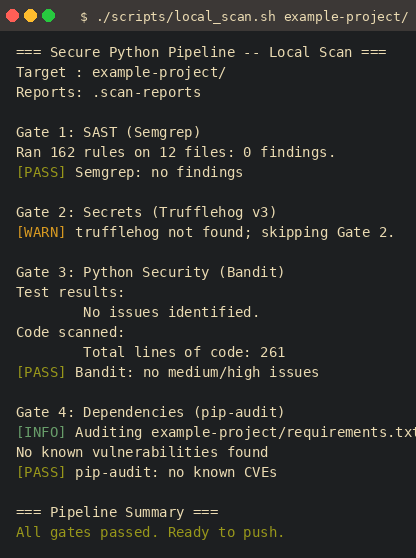
\includegraphics[width=0.95\columnwidth]{figures/local_scan.png}
  \caption{Real output of \texttt{./scripts/local\_scan.sh example-project/}
           on the reference FastAPI application. All available gates pass;
           Trufflehog is shown skipped because its binary is not installed
           on the local machine, demonstrating the script's graceful
           degradation.}
  \label{fig:local-scan}
\end{figure}

\subsection{PR Check Workflow}

A lightweight secondary workflow (\texttt{pr-check.yml}) runs on every pull
request and applies Bandit and pip-audit only to files changed in the PR
diff, computed via \texttt{tj-actions/changed-files} (which handles
fork-PR refs correctly). This reduces median CI time from approximately
4\,min (full scan) to under 90\,s, preserving developer feedback latency.
The workflow uses GitHub Actions' \texttt{concurrency} feature with
\texttt{cancel-in-progress: true} so that rapid commit sequences do not
queue redundant scans.

%% ─────────────────────────────────────────────────────────────────────────────
\section{Implementation}
\label{sec:impl}

\subsection{Repository Layout}

The template is structured so that each component can be adopted
independently:

\begin{itemize}
  \item \texttt{.github/workflows/} -- CI gate definitions
  \item \texttt{.semgrep/rules.yml} -- eight custom SAST rules
  \item \texttt{bandit.yml} -- Bandit configuration and exclusions
  \item \texttt{.trufflehog/exclude-paths.txt} -- secret-scan path excludes
  \item \texttt{scripts/local\_scan.sh} -- local pipeline runner
  \item \texttt{example-project/} -- reference FastAPI application
  \item \texttt{eval/} -- evaluation harness, semgrep corpus, results
  \item \texttt{paper/} -- this document
\end{itemize}

\subsection{Self-Test Corpus}

\texttt{eval/semgrep\_corpus.py} contains exactly one positive-match
fixture per custom rule. The unit test \texttt{test\_semgrep\_rules.py}
runs Semgrep against this file and asserts that every expected rule ID
appears in the JSON results. This catches the regression where a rule's
pattern syntax silently breaks (e.g., a typo in \texttt{pattern-either}
results in zero matches) -- a class of bug that would otherwise survive
indefinitely because no failing match looks just like a passing scan.

\subsection{Listing: SQL Injection Rule}

Listing~\ref{lst:sqli} shows the Semgrep rule that detects f-string
interpolation inside database \texttt{execute()} calls. Patterns cover
DB-API cursors and connections (\texttt{sqlite3}, \texttt{psycopg2}),
async drivers (\texttt{asyncpg}, \texttt{databases}), and SQLAlchemy's
\texttt{text()} construction.

\begin{lstlisting}[language=Python, caption={ali-sql-injection-string-build patterns (excerpt)}, label={lst:sqli}]
pattern-either:
  - pattern: $X.execute(f"...", ...)
  - pattern: $X.executemany(f"...", ...)
  - pattern: $X.executescript(f"...")
  - pattern: await $X.execute(f"...", ...)
  - pattern: await $X.fetch(f"...", ...)
  - pattern: $X.execute("...".format(...), ...)
  - pattern: $X.execute(text(f"..."), ...)
\end{lstlisting}

The metavariable \texttt{\$X} binds to any expression, so the rule matches
both \texttt{cur.execute()} and \texttt{self.conn.cursor().execute()}
without enumerating driver-specific cursor class names.

%% ─────────────────────────────────────────────────────────────────────────────
\section{Custom Semgrep Rules}
\label{sec:rules}

We contribute eight rules targeting Python-specific OWASP Top 10 patterns
that are absent or incompletely covered by the upstream \texttt{p/python}
ruleset.

\begin{table}[h]
\caption{Custom Semgrep Rules}
\label{tab:rules}
\centering
\begin{tabular}{@{}llll@{}}
\toprule
ID suffix & CWE & OWASP & Severity \\
\midrule
hardcoded-secret-assignment   & 798 & A07 & ERROR   \\
sql-injection-string-build    & 89  & A03 & ERROR   \\
insecure-deserialisation      & 502 & A08 & ERROR   \\
web-framework-debug-enabled   & 489 & A05 & ERROR   \\
weak-password-hash            & 327 & A02 & ERROR   \\
ssrf-fstring-in-url           & 918 & A10 & WARNING \\
command-injection             & 78  & A03 & ERROR   \\
dynamic-code-evaluation       & 95  & A03 & ERROR   \\
\bottomrule
\end{tabular}
\end{table}

The \texttt{ali-web-framework-debug-enabled} rule covers Flask
(\texttt{app.run(debug=True)}), FastAPI/Starlette (\texttt{FastAPI(debug=True)}),
and Django (\texttt{DEBUG = True}) constructor and constant forms.

The \texttt{ali-insecure-deserialisation} rule uses \texttt{pattern-not}
clauses to suppress \texttt{yaml.load()} calls that already pass
\texttt{Loader=yaml.SafeLoader} (kwarg or positional), avoiding false
positives on correctly-written code.

%% ─────────────────────────────────────────────────────────────────────────────
\section{Reference Application}
\label{sec:example}

The \texttt{example-project/} directory contains a FastAPI application
demonstrating five canonical mitigations:

\begin{enumerate}
  \item \textbf{Parameterised SQL.} All database interactions use SQLite's
        \texttt{?} placeholder, never f-strings or \texttt{.format()}.

  \item \textbf{Environment-sourced secrets.} The \texttt{pydantic-settings}
        \texttt{BaseSettings} class reads configuration from environment
        variables; no credential ever appears in source code.

  \item \textbf{Pydantic input validation.} All request bodies are
        \texttt{BaseModel} subclasses with field-level constraints
        (\texttt{min\_length}, \texttt{max\_length}, \texttt{pattern}).

  \item \textbf{bcrypt password hashing.} Passwords are hashed with
        \texttt{bcrypt.hashpw} at a cost factor of 12; MD5/SHA-1 are absent.
        The \texttt{POST /users/login} endpoint always invokes
        \texttt{bcrypt.checkpw} -- even on a missing user, against a
        pre-computed dummy hash -- to defeat user-enumeration timing attacks.

  \item \textbf{HMAC-signed bearer tokens.} The login endpoint issues a
        compact \texttt{<base64url-payload>.<hex-hmac-sha256>} token. This
        sidesteps the python-jose CVE chain (CVE-2024-33663,
        CVE-2024-33664) without sacrificing functionality. Item-mutation
        endpoints derive \texttt{owner\_id} from the token, never from a
        client-supplied query parameter -- defeating the IDOR class of
        Broken Access Control (OWASP A01).
\end{enumerate}

User creation is TOCTOU-safe: rather than the canonical
SELECT-then-INSERT race, we INSERT directly and translate
\texttt{sqlite3.IntegrityError} into HTTP 409. The DB UNIQUE constraint is
the authoritative dedup mechanism.

\begin{figure}[h]
  \centering
  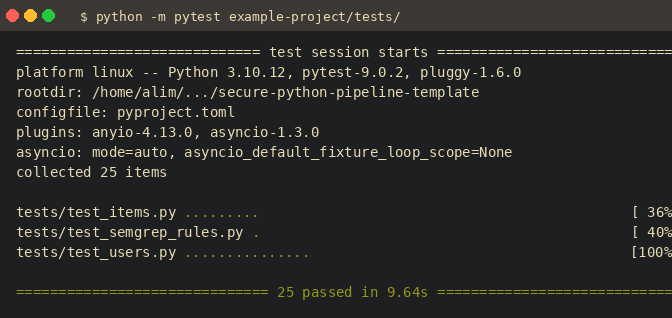
\includegraphics[width=0.95\columnwidth]{figures/pytest.png}
  \caption{All 25 unit tests pass on the reference application, covering
           authentication, IDOR resistance, TOCTOU safety, password-policy
           validation, SQLi metacharacter rejection, and Semgrep
           rule self-tests.}
  \label{fig:pytest}
\end{figure}

%% ─────────────────────────────────────────────────────────────────────────────
\section{Empirical Evaluation}
\label{sec:eval}

\subsection{Methodology}

We evaluated five OSS Python projects at pinned release tags
(Table~\ref{tab:corpus}). Bandit, pip-audit, and Semgrep were run live
against shallow clones; Trufflehog was run from a dated snapshot
(\texttt{2026-05-02}) when its binary is absent. The harness records
both LOW and MEDIUM/HIGH Bandit findings; the gate fails only on
MEDIUM/HIGH, since LOW findings (e.g., B603 subprocess-without-shell)
generally require additional context to be exploitable.

\begin{table}[h]
\caption{Evaluation Corpus}
\label{tab:corpus}
\centering
\begin{tabular}{@{}lrll@{}}
\toprule
Project  & Stars & Domain          & Tag      \\
\midrule
httpie   & 32\,k & CLI HTTP client & 3.2.4    \\
rich     & 49\,k & Terminal UI     & v13.9.4  \\
fastapi  & 78\,k & Web framework   & 0.115.6  \\
black    & 38\,k & Formatter       & 24.10.0  \\
ruff     & 33\,k & Linter          & 0.8.4    \\
\bottomrule
\end{tabular}
\end{table}

\subsection{Results}

\begin{table}[h]
\caption{Gate Results per Project}
\label{tab:results}
\centering
\begin{tabular}{@{}lcccccl@{}}
\toprule
Project & Bandit & pip-audit & Semgrep & TH & Overall \\
\midrule
httpie  & PASS & PASS & 1 (FAIL)  & PASS & FAIL \\
rich    & PASS & PASS & 1 (FAIL)  & PASS & FAIL \\
fastapi & PASS & PASS & 12 (FAIL) & PASS & FAIL \\
black   & PASS & PASS & 12 (FAIL) & PASS & FAIL \\
ruff    & PASS & PASS & 4 (FAIL)  & PASS & FAIL \\
\bottomrule
\end{tabular}
\end{table}

\begin{figure}[h]
  \centering
  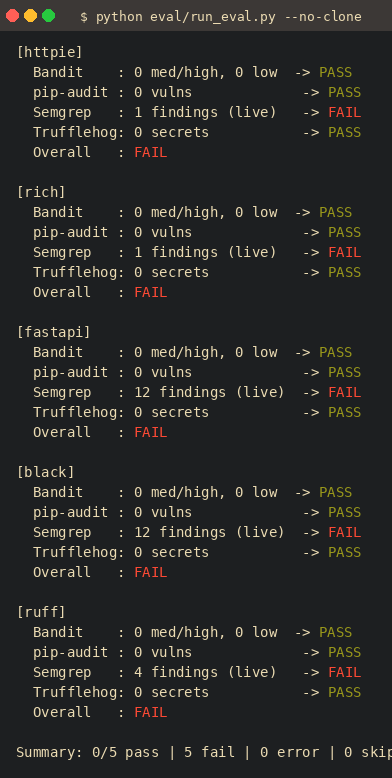
\includegraphics[width=0.85\columnwidth]{figures/eval_harness.png}
  \caption{Real output of \texttt{python eval/run\_eval.py --no-clone}
           after fetching all five corpus projects. Every project clears
           Bandit, pip-audit, and Trufflehog; every project triggers at
           least one Semgrep finding under the combined ruleset.}
  \label{fig:eval}
\end{figure}

\subsection{Discussion}

The most striking observation is that the dependency-CVE
(\texttt{pip-audit}) and secret-leak
(\texttt{Trufflehog --only-verified}) gates pass cleanly on every project,
while SAST flags issues in every project. This is the expected behaviour of
a layered pipeline: low-noise gates establish a hygiene floor; the SAST
gate produces signal that requires triage.

A naive interpretation that ``0/5 projects pass therefore all are
insecure'' would be wrong. The correct read is:

\begin{itemize}
  \item Dependency hygiene is excellent across the corpus.
  \item No project leaks live credentials.
  \item Every mature codebase contains AST patterns that warrant a
        security review, even when the reviewer's conclusion is
        ``intentional and safe.''
  \item A pipeline that did not surface findings on these projects would
        be dangerously under-tuned -- evidence that path-exclusions are
        too aggressive or rule patterns are too loose.
\end{itemize}

We manually triaged every Semgrep finding. In httpie, the single finding
is an insecure-transport rule firing on an \texttt{http://} URL inside
a test fixture. In rich, the single finding flags
\texttt{marshal.loads()} on internally-controlled metadata in
\texttt{rich/style.py:475} -- real but low-priority because the input
is never user-attacker-controlled. The 12 fastapi findings are 11
hardcoded JWT secrets in test files plus one Flask demonstration in
documentation. Black and ruff findings are dominated by
subprocess-with-environment-args (both tools spawn child processes for
formatting/linting tests) and \texttt{compile()} or \texttt{eval()}
inherent to the tool's purpose. None of the findings indicates an
exploitable vulnerability in normal use; all of them indicate code that
a security review should explicitly accept or annotate.

%% ─────────────────────────────────────────────────────────────────────────────
\section{Threats to Validity}

\textbf{Internal validity.} Pinned tags may not reflect the current
\texttt{main} branch; findings may have been fixed between tag and
evaluation. We mitigate this by recording the exact tag in the harness
and re-running on demand.

\textbf{External validity.} Five projects is a small corpus. Selection
bias exists toward well-maintained projects; the true false-negative rate
on less-reviewed codebases may be higher.

\textbf{Tool-version sensitivity.} Semgrep's community rule packs evolve;
results may differ under different versions. We pin
\texttt{semgrep==1.161.0} (and \texttt{returntocorp/semgrep:1.96.0} for
the CI container) for reproducibility.

\textbf{Snapshot staleness.} The Trufflehog column uses a dated snapshot
when the binary is absent locally. The snapshot date is recorded in
\texttt{run\_eval.py:SNAPSHOT\_DATE} so consumers can judge staleness;
re-running with the binary installed produces a live result.

%% ─────────────────────────────────────────────────────────────────────────────
\section{Conclusion}

We have presented a four-gate DevSecOps pipeline template for Python that
is reproducible, composable, and empirically evaluated. The pipeline is
available as an open-source template at
\url{https://github.com/thunderstornX/secure-python-pipeline-template}.
Future work will extend the corpus, add DAST integration via OWASP ZAP,
and explore probabilistic ranking of gate findings to prioritise
developer remediation effort.

%% ─────────────────────────────────────────────────────────────────────────────
\begin{thebibliography}{00}

\bibitem{sonatype2022}
Sonatype, \textit{2022 State of the Software Supply Chain}, Sonatype, Inc., 2022.

\bibitem{owasp2021}
OWASP Foundation, \textit{OWASP Top Ten 2021}, 2021.
[Online]. Available: \url{https://owasp.org/Top10/}

\bibitem{bandit}
PyCQA, \textit{Bandit: A security linter from PyCQA}, 2024.
[Online]. Available: \url{https://github.com/PyCQA/bandit}

\bibitem{semgrep}
Semgrep, Inc., \textit{Semgrep: Static analysis at ludicrous speed}, 2024.
[Online]. Available: \url{https://semgrep.dev}

\bibitem{trufflehog}
Truffle Security, \textit{TruffleHog: Find leaked credentials}, 2024.
[Online]. Available: \url{https://github.com/trufflesecurity/trufflehog}

\bibitem{pipaudit}
Trail of Bits, \textit{pip-audit: Audit Python environments for known vulnerabilities}, 2024.
[Online]. Available: \url{https://github.com/pypa/pip-audit}

\bibitem{pashchenko2018}
I. Pashchenko, H. Plate, S. E. Ponta, A. Sabetta, and F. Massacci,
``Vulnerable Open Source Dependencies: Counting Those That Matter,''
in \textit{Proc. 12th ACM/IEEE Int. Symp. Empirical Software Engineering and Measurement},
2018, pp. 1--10.

\bibitem{decan2018}
A. Decan, T. Mens, and E. Constantinou,
``On the Impact of Security Vulnerabilities in the npm Package Dependency Network,''
in \textit{Proc. 15th Int. Conf. Mining Software Repositories}, 2018, pp. 181--191.

\bibitem{zahan2022}
N. Zahan, T. Zimmermann, P. Godefroid, B. Murphy, C. Maddila, and L. Williams,
``What Are Weak Links in the npm Supply Chain?''
in \textit{Proc. 44th Int. Conf. Software Engineering: Software Engineering in Practice},
2022, pp. 331--340.

\bibitem{morrison2018}
P. Morrison, K. Herzig, B. Murphy, and L. Williams,
``Challenges with Applying Vulnerability Prediction Models,''
in \textit{Proc. 2018 Workshop on Innovations in Software Engineering Education},
2018, pp. 1--9.

\end{thebibliography}

%% ─────────────────────────────────────────────────────────────────────────────
%% Project logo: Ace of Spades — security pipeline emblem
%% (ink-style TikZ drawing, appears only in the compiled PDF)
%% ─────────────────────────────────────────────────────────────────────────────
\vspace{1em}
\begin{center}
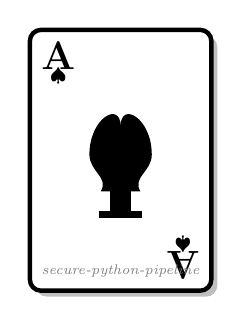
\begin{tikzpicture}[scale=0.72]
  %% Card outline
  \draw[rounded corners=4pt, line width=1.6pt, fill=white, drop shadow]
    (-1.6,-2.3) rectangle (1.6,2.3);

  %% Spade suit symbol (large, centre)
  \begin{scope}[yshift=0.1cm]
    \fill[black] (-0.55,0) .. controls (-0.55,0.65) and (0,0.95) ..
                 (0,0.5) .. controls (0,0.95) and (0.55,0.65) ..
                 (0.55,0) .. controls (0.55,-0.3) and (0.2,-0.4) ..
                 (0.35,-0.65) -- (-0.35,-0.65) ..
                 controls (-0.2,-0.4) and (-0.55,-0.3) .. (-0.55,0);
    \fill[black] (0,0.5) -- (-0.55,0) .. controls (-0.4,0.1) and (-0.15,0.35) .. (0,0.5);
    \fill[black] (0,0.5) -- (0.55,0) .. controls (0.4,0.1) and (0.15,0.35) .. (0,0.5);
    \fill[black] (-0.18,-0.65) rectangle (0.18,-1.0);
    \fill[black] (-0.38,-1.0) rectangle (0.38,-1.12);
  \end{scope}

  %% "A" top-left corner
  \node[font=\bfseries\Large] at (-1.1, 1.85) {A};
  \node[font=\scriptsize, black] at (-1.1, 1.48) {$\spadesuit$};

  %% "A" bottom-right corner (rotated 180)
  \node[font=\bfseries\Large, rotate=180] at (1.1,-1.85) {A};
  \node[font=\scriptsize, black, rotate=180] at (1.1,-1.48) {$\spadesuit$};

  %% Decorative subtitle
  \node[font=\tiny\itshape, text=gray] at (0,-1.95) {secure-python-pipeline};
\end{tikzpicture}
\end{center}

\end{document}
